\documentclass{article}
\usepackage{blindtext}
\usepackage[utf8]{inputenc}
\usepackage{subfiles}
\usepackage{ragged2e}
\usepackage{biblatex}
\usepackage[a4paper, total={6.2in, 8.9in}]{geometry}

\usepackage{listings}
\usepackage[pdftex]{graphicx}
    \graphicspath{./images}
    \DeclareGraphicsExtensions{.pdf, .png}

% commands
\renewcommand{\arraystretch}{1.5}
\renewcommand{\labelitemi}{$\textendash$}
\addbibresource{report.bib}

\author{Arumoy Shome & Shruti Rao}
\date{20 October, 2018}

\begin{document}
% \maketitle
\begin{titlepage}
    \begin{center}
        \vspace*{1cm}
        
        \huge
        
        \textbf{Movable Patient Support for an MRI Scanner}
        \vspace{1.5cm}
        
        \textbf{Arumoy Shome \& Shruti Rao}
        
        \vfill
        
        A Report Submitted in Partial Fullfillment of the 
        
        Requirements for Protocol Valication
        
        \vspace{0.8cm}
        
        \large
        Computer Science\\
        Vrije Universiteit\\
        Netherlands\\
        October 20, 2018
    \end{center}
\end{titlepage}
%%%%% Preamble to the document ends here %%%%%%

\newpage
\thispagestyle{empty}
\tableofcontents
\newpage
\thispagestyle{empty}
\listoffigures
\newpage
\thispagestyle{empty}
\listoftables
\pagenumbering{arabic}

\newpage
\section{Introduction}
Magnetic Resonance Imaging (MRI) Scanners are used primarily in the medical field to produce images of patient tissues\cite{yanke_haken_aisen_fraass_thornton_1991}. This assignment consists of designing controllers for a movable patient support unit that is part of a larger MRI system. The Patient Support unit as described by this assignment is used to move patients in and out of the MRI scanner.

% TODO: Rewrite order as per final report
The report begins by identifying and discussing the global requirements of the system in natural language. Next, the global properties are restated using pre-defined interaction terms. A system architecture is presented to help visualize the control system and all interactions are verified using mcrl2 code\cite{mcrl2}. 

%TODO: Add assumption about isCalibrated
\section{System Specifications}
Figure \ref{fig:pss} represents the Movable Patient Support Unit (MPSU) that we aim to model for. The goal is to ensure that no harm can ever be done to the patient or the equipment. The most important safety requirement is implemented in hardware so the emergency button prevents any motors from being engaged and allows manual operation to take over.

Other safety requirements are implemented in the software and concerns the movements of the bed. The bed cannot move further than the defined extremes to prevent it from tumbling. The motors and their corresponding breaks cannot work at the same time to prevent overheating. The bed can be undocked only when it is completely outside the scanner. Finally, the bed must only be allowed to move when it is docked and calibrated. It must not be allowed to move when undocked \cite{ponse}. The MPSU can be controlled with the help of a Console shown in figure \ref{fig:console}.

\begin{figure}[!h]
    \centering
    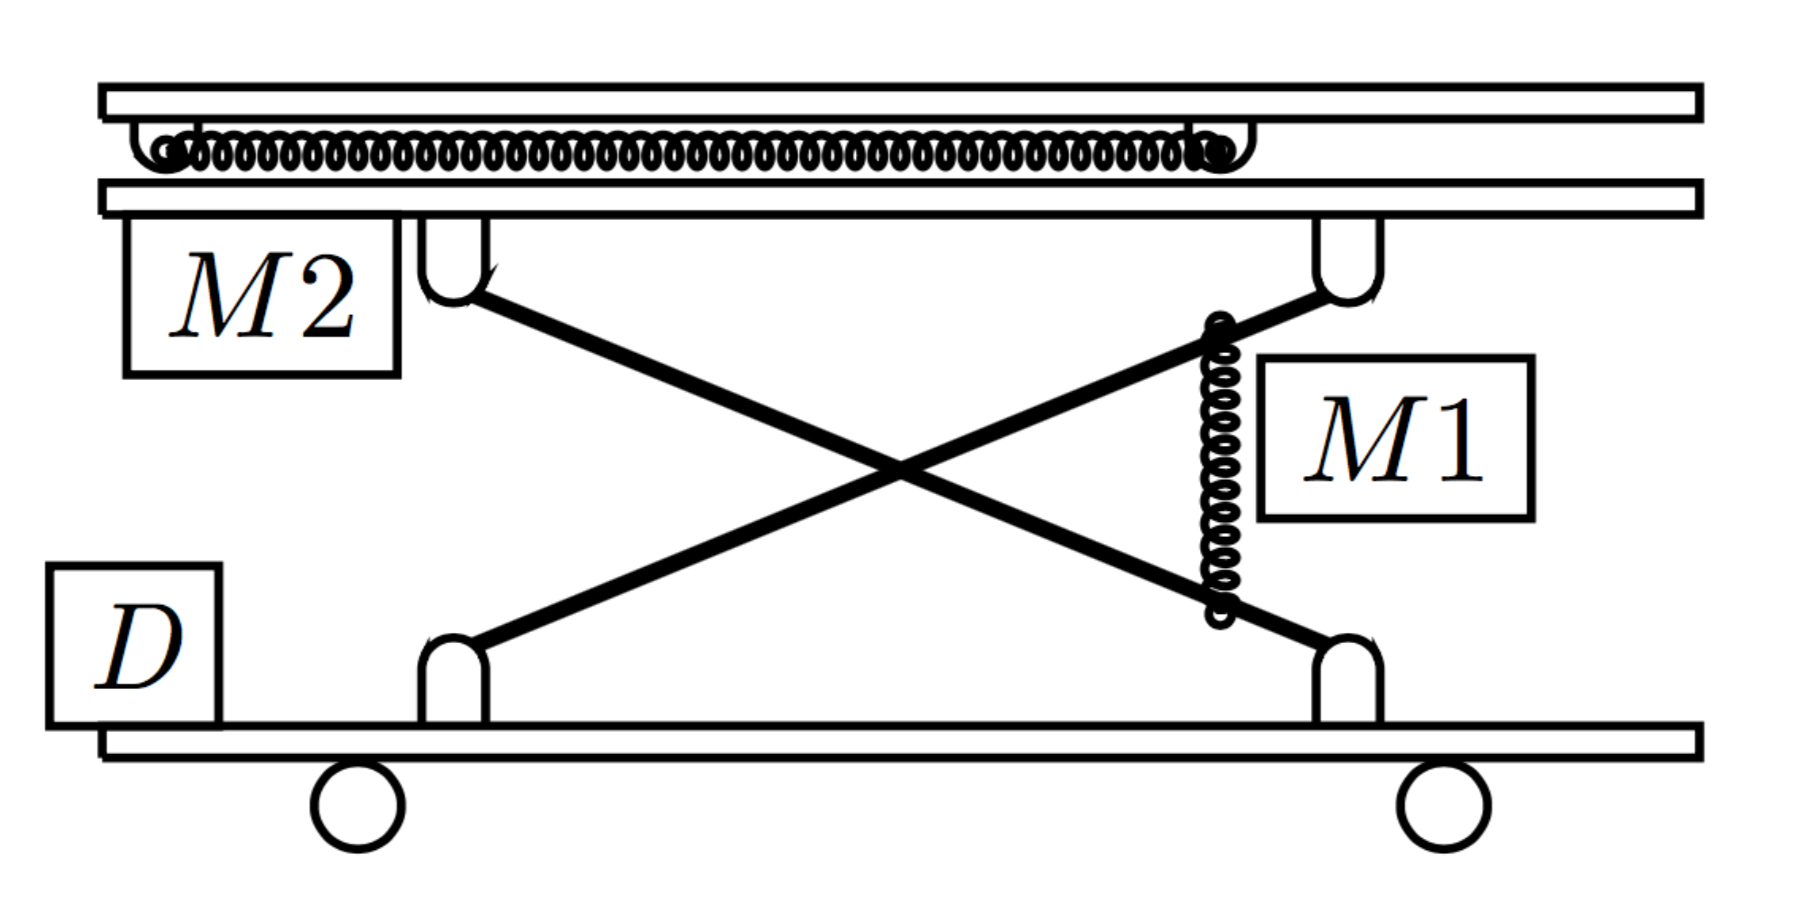
\includegraphics[width=\textwidth]{images/pss.png}
    \caption{Patient Support System}
    \label{fig:pss}
\end{figure}

\begin{figure}[!h]
    \centering
    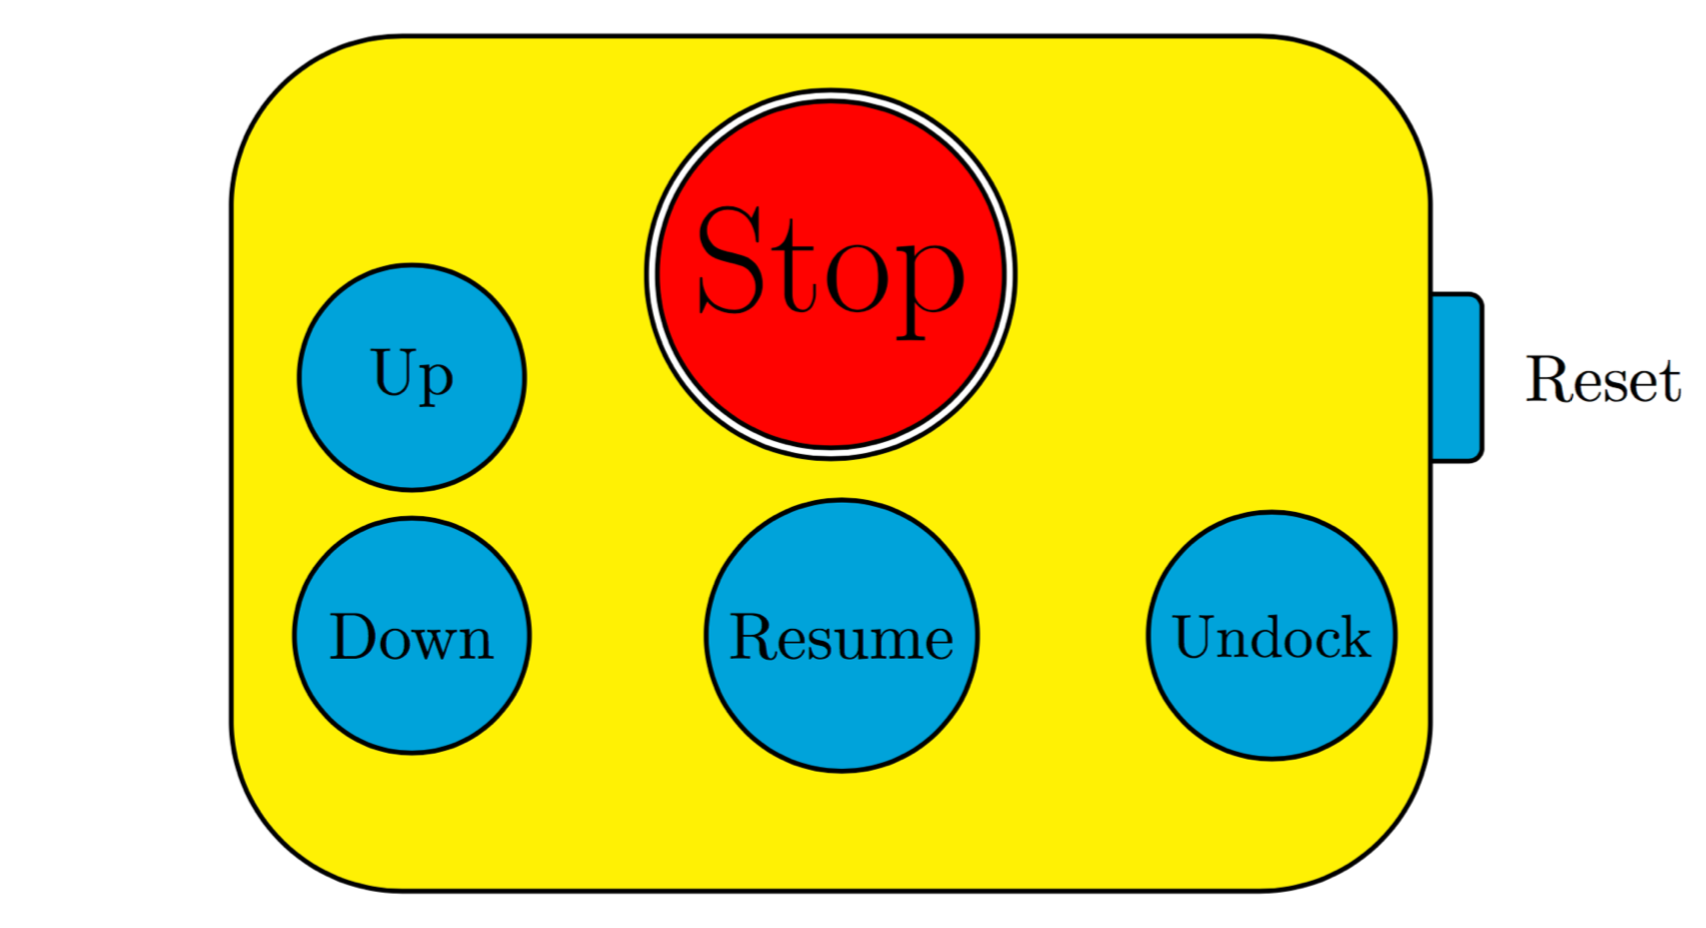
\includegraphics[width=14.7cm]{images/console.png}
    \caption{Console for Patient Support System}
    \label{fig:console}
\end{figure}


Three separate controllers (as depicted in figure \ref{fig:sysarch} are used to model the system. For the purposes of this assignment, we assume that the controllers communicate with each other in a lossless manner \cite{ponse}.

\begin{itemize}
    \item [\textbullet] \textit{Console} receives input from the user interface and passes that information to the \textit{Sensor}. 
    \item [\textbullet] \textit{Sensor} keeps track of the mode in which the MPSU is operating in (Emergency or Normal mode) and whether it is docked and calibrated.
    It receives input from various sensors for detecting movement of the bed at the outermost, innermost, topmost and bottom most positions. Based on the sensor information and input from the \textit{Console}, it instructs the \textit{Hardware} on what to do next.
    \item [\textbullet] \textit{Hardware} is responsible for the vertical and horizontal movements of the MPSU. Based on the instructions received from the \textit{Sensor}, it triggers certain sets of actions on the breaks and motors.
\end{itemize}
 
\begin{figure}[h]
\centering
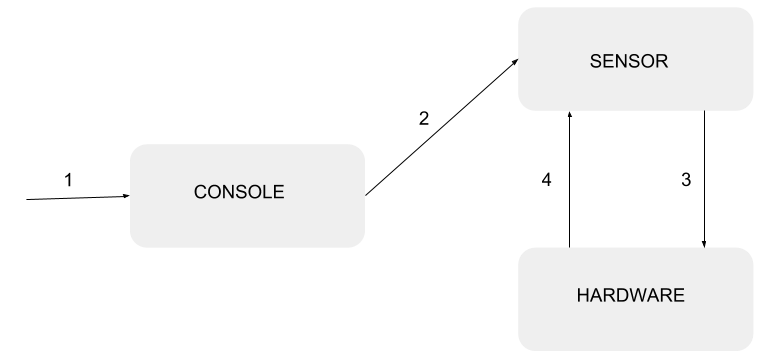
\includegraphics[width=\textwidth]{images/system-architecture.png}
\caption{System Architecture}
\label{fig:sysarch}
\end{figure}

\newpage
\section{Interaction Terms}
To understand the behaviour of the controllers, its interactions are listed as behavioural properties. These properties are categorized by the controller they define, so Table \ref{table:1} lists all the interactions of the \textit{Hardware} controller. Table \ref{table:2} holds all the interactions associated with \textit{Console}, while Table \ref{table:3} defines the interactions for \textit{Sensor}.

\begin{table}[!h]
\centering
\begin{tabular}{ |l|l| } 
	\hline
	\textbf{Interactions} & \textbf{Description}\\
	\hline
    \texttt{m2Left} & Motor2 is switched on and moves bed left\\
    \texttt{m2Right} & Motor2 is switched on and moves bed right\\
	\texttt{m2Off} & Turn off Motor2\\
	\texttt{m1Up} & Motor1 is switched on and moves bed up\\
    \texttt{m1Down} & Motor2 is switched on and moves bed down\\
    \texttt{m1Off} & Turn off Motor1\\
	\texttt{applyBreak1} & Applies vertical break preventing bed from moving\\
	\texttt{releaseBreak1} & Releases vertical break allowing bed to move\\
	\texttt{applyBreak2} & Applies horizontal break preventing bed from moving\\
	\texttt{releaseBreak2} & Releases horizontal break allowing bed to move\\
	\hline
\end{tabular}
\caption{List of Hardware Interactions}
\label{table:1}
\end{table}

\begin{table}[h]
\centering
\begin{tabular}{ |l|l| } 
    \hline
	\textbf{Interactions} & \textbf{Description} \\
    \hline
    \texttt{pressUp} & The Up button is pressed\\
	\texttt{pressDown} & The Down button is pressed\\
	\texttt{unlockDock} & Unlocks the bed from the unit\\
	\texttt{pressStop} & Stop button is pressed that turns on Emergency mode\\
    \texttt{pressResume} & the Resume button is pressed which turns off Emergency mode\\
	\texttt{pressUndock} & The Undock button is pressed that undocks the bed\\
	\texttt{pressReset} & The Reset button is pressed that resets ths calibrated height\\
	\hline
\end{tabular}
\caption{List of Console Interactions}
\label{table:2}
\end{table}

\begin{table}
\centering
\begin{tabular}{ |l|l| } 
	\hline
	\textbf{Interactions} & \textbf{Description}\\
	\hline
	\texttt{isDocked} & Indicates that the bed is docked to scanner\\
	\texttt{isCalibrated} & Indicates that the bed is at standard height\\
	\texttt{atTopMost} & Bed is at the top most height or standard height\\
	\texttt{atBottomMost} & Bed is at the lowest height\\
	\texttt{atLeftMost} & Bed is completely inside the scanner\\
	\texttt{atRightMost} & Bed is completely outside the scanner\\
	\hline
\end{tabular}
\caption{List of Sensor Interactions}
\label{table:3}
\end{table}

\newpage
\section{System Requirements}
\begin{enumerate}
    \item Motor should not be running if bed is at extremes
    
    \texttt{m2Left} cannot occur after \texttt{atLeftMost} has occurred. \texttt{m2Right} cannot occur \texttt{atRightMost} has occurred. \texttt{m1Up} cannot occur after \texttt{atTopMost} has occurred. \texttt{m1Down} cannot occur after \texttt{atBottomMost} has occurred
    \begin{itemize}
        \item [\textendash] $[atLeftMost^{\ast}.m2Left]False$
        \item [\textendash] $[atRightMost^{\ast}.m2Right]False$
        \item [\textendash] $[atRightMost^{\ast}.m2Right]False$
        \item [\textendash] $[atTopMost^{\ast}.m1Up]False$
        \item [\textendash] $[atBottomMost^{\ast}.m1Down]False$
    \end{itemize}


    \item System should not tumble over
    
    \texttt{unlockDock} must be preceeded by \texttt{atRightMost}, \texttt{applyBreak2} and \texttt{m2Off}. Between \texttt{unlockDock} and \texttt{atRightMost}, no \texttt{m2Left} should occur.Between \texttt{unlockDock} and \texttt{m2Off}, no \texttt{m2Left} or \texttt{m2Right} should occur. Between \texttt{unlockDock} and \texttt{applyBreak2}, no \texttt{releaseBreak2} should occur.

    \begin{itemize}
        \item [\textendash] $[T ^{\ast}.m2Left.(\neg atRightMost)^{\ast}.unlockDock]False$
        \item [\textendash] $[T ^{\ast}.(m2Left \wedge m2Right).(\neg m2Off) ^{\ast}.unlockDock]False$
        \item [\textendash] $[T ^{\ast}.releaseBreak1.(\neg applyBreak1)^{\ast}.unlockDock]False$
        \item [\textendash] $[(\neg atRightMost)^{\ast}.unlockDock]False$
        \item [\textendash] $[(\neg applyBreak2)^{\ast}.unlockDock]False$
        \item [\textendash] $[(\neg m2Off)^{\ast}.unlockDock]False$
    \end{itemize}
    
    \item During normal operation, if a motor is on, then it's brake must not be applied and vice versa.
    
    \texttt{applyBreak1} and \texttt{applyBreak2} must be preceeded by \texttt{M1Off} and \texttt{M2Off} respectively. Furthermore, \texttt{ApplyBreak1} cannot be followed by \texttt{Motor1Off}, unless \texttt{ReleaseBreak1} has occured between the two events. The same is true for Motor 2 as well.
    
    \begin{itemize}
        \item [\textendash] $[\neg m1Off.T^{\ast}.applyBreak1]F$
        \item [\textendash] $[\neg m2Off.T^{\ast}.applyBreak2]F$
        \item [\textendash] $[T^{\ast}.applyBreak1.(\neg releaseBreak1)^{\ast}.\neg m1Off]F$
        \item [\textendash] $[T^{\ast}.applyBreak2.(\neg releaseBreak2)^{\ast}.\neg m2Off]F$
    \end{itemize}
    
    \item The Stop button when pressed activates Emergency Mode
    
    \texttt{pressStop} must be immediately followed by \texttt{releaseBreak2}, \texttt{m2Off}, and \texttt{unlockDock} and no actions should occur between \texttt{pressStop} and any of \texttt{releaseBreak2}, \texttt{m2Off} and \texttt{unlockDock}
    
    \begin{itemize}
        \item [\textendash] $[T^{\ast}.pressStop].\mu X[\neg releaseBreak2]X$
        \item [\textendash] $[T^{\ast}.pressStop].\mu X[\neg m2Off]X$
        \item [\textendash] $[T^{\ast}.pressStop].\mu X[\neg unlockDoc]X$
    \end{itemize}
        
    \item Resume button undoes Emergency mode
    
    \texttt{pressResume} must be preceeded by \texttt{isDocked}
    \begin{itemize}
        \item [\textendash] $[T^{\ast}(pressStop \wedge isDocked).<T>T.pressResume].\mu X[\neg appyBreak2]X$
    \end{itemize}

    \item Bed can be not docked only when in outermost position and brake is applied
    
    \texttt{pressUndock} must be preceeded by \texttt{atRightMost} and between them \texttt{m2Left} or \texttt{releaseBreak2} must not have occurred
    \begin{itemize}
        \item [\textendash] $[T^{\ast}.atOuterMost.(\neg m2Left \vee \neg releaseBreak2).pressUndock].\mu X[\neg unlockDock]X$
    \end{itemize}


    \item While docked the reset button when pressed after setting the scanner height, calibrates the height
    
    \texttt{pressReset} must be preceeded by \texttt{isDocked} and any \texttt{m1Up} and \texttt{m1Down} may occur in between. \texttt{isCalibrated} must follow and there must be no occurrence of \texttt{m2Left} and \texttt{m2Right}
    \begin{itemize}
        \item [\textendash] $[T^{\ast}.isDocked].\mu X(\neg m2Left \vee \neg m2Right) \wedge [\neg pressReset]X).\mu X[\neg isCalibrated]X$
    \end{itemize}
    
    
    \item Pressing reset button when not docked, uncalibrates the system

    If \texttt{isCalibrated} is eventually followed by \texttt{unlockDock} and \texttt{pressRese}t occurs then \texttt{isCalibrated} must follow
    \begin{itemize}
        \item [\textendash] $[T^{\ast}.isCalibrated].\mu X(<T>T \vee [\neg unlockDock \vee \neg pressReset]X).\mu X[\neg isCalibrated]X$
    \end{itemize}


    \item While docked and calibrated, the Up button moves the bed inside the scanner
        
    After \texttt{isDocked} and \texttt{isCalibrated} actions occur, \texttt{pressUp} is immediately followed by \texttt{M2Left} till \texttt{atLeftMost} is reached
        
    \begin{itemize}
            \item [\textendash]$[T ^{\ast}.isCalibrated \wedge isDocked] <pressUp>.\muX(m2Left \wedge [\neg atLeftMost]X)$
    \end{itemize}

    \item While docked and calibrated, pressing the Down button moves the bed outside of the scanner
    
    After \texttt{isDocked} and \texttt{isCalibrated} occur, \texttt{pressDown} is immediately followed by \texttt{m2Right} till \texttt{atRightMost} occurs.
    
    \begin{itemize}
        \item [\textendash]$[T {\ast}.(isDocked \vee isCalibrated).<pressDown>.\muX(m2Right \wedge [\neg atRightMost]X)$
    \end{itemize}

    \item While not docked and not calibrated, pressing the Up button moves the bed up
        
    If \texttt{isDocked} and \texttt{isCalibrated} have not occured, \texttt{pressUp} is immediately followed by \texttt{m1Up} till \texttt{atTopMost} occurs.
    
    \begin{itemize}
        \item [\textendash] $[T ^{\ast}.\neg isCalibrated \wedge \neg isDocked] <pressUp>.\muX(m1Up \wedge [\neg atTopMost]X)$
    \end{itemize}
    
    \item While not docked and not calibrated, pressing the Down button moves the bed down
    
    If \texttt{isDocked} and \texttt{isCalibrated} have not occured, \texttt{pressDown} is immediately followed by \texttt{m1Down} till \texttt{atBottomMost} occurs.
    
    \begin{itemize}
        \item [\textendash] $[T ^{\ast}.\neg isCalibrated \wedge \neg isDocked] <pressDown>.\muX(m1Down \wedge [\neg atBottomMost]X)$
    \end{itemize}
\end{enumerate}

\section{Code Listing}
\lstinputlisting{mpsu-parallel.mcrl2}

\newpage
\printbibliography
\end{document}
